\section{Methods}
\vspace{-0.5cm}
\subsection{Nitrite Investigations}
\vspace{-0.5cm}
To obtain the voltammogram and calibration curves, DPV was performed on increasing concentrations of nitrite solution using the apparatus as described in \autoref{fig:h2o2_setup}. The solution was degassed with nitrogen gas to remove oxygen gas.\\
\begin{table}[H]
    \centering
    \begin{tabular}{ |p{3.7cm}||p{3.7cm}| } 
        \hline
        \multicolumn{2}{|l|}{\textbf{Reusable gold electrode}} \\ \hline
        Reusable gold electrode in PBS solution & Obtain baseline voltammetry and calibration curve for nitrite detection and estimate expected peaks\\ \hline
        Reusable gold electrode with 4\% albumin & Determine magnitude of effect of albumin in solution and compare to previous results \\ \hline
        \multicolumn{2}{|l|}{\textbf{Disposable gold electrode}} \\ \hline
    Disposable gold electrode in PBS solution & Obtain voltammetry and calibration curve and compare performance to reusable electrodes. \\ \hline
    Disposable gold electrode with 5.2g/L albumin & Determine magnitude of effect of albumin in solution and compare to previous results\\ \hline
    \end{tabular}
    \caption{A summary of performed experiments is shown}
    \label{tab:my_label}
\end{table}

\noindent{Detailed descriptions of performed experiments are listed in \autoref{app:nitrite_protocol}.}



\begin{figure}[H]
\centering
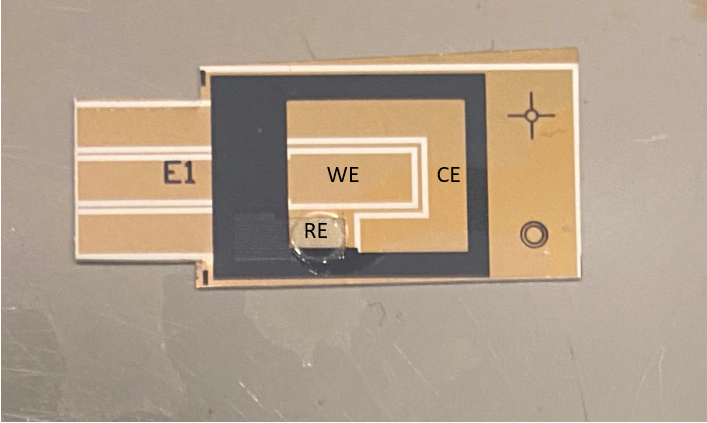
\includegraphics[width=0.45\textwidth]{img/disp electrode.PNG}
\caption{Image of gold disposable electrode. Working electrode (WE), Reference electrode (RE), Counter electrode (CE). pHEMA layer has been applied to RE. Disposable electrodes were prepared by washing in 75\% ethanol, and the RE was coated with 5$\mu$M Polyhydroxyethylmethacrylate (pHEMA) and baked for one hour at 70\textdegree{C}}
\end{figure}


\subsection{Hydrogen Peroxide Investigations}
To perform the sensing of hydrogen peroxide with Prussian blue, a four-step protocol has been established based on the publication by Chen \textit{et al.} \cite{C9AN02438G}, as shown in \autoref{app:h2o2_protocol}. Gold (Au) electrode were adopted for the calibration in the current stage. However disposable electrodes may be introduced for blood sample testing in the future work. \\\\
In the first stage of electrochemical detection, the PEDOT:PSS-PB complex has been synthesised and crosslinked with ethylene glycol (EG) and  divinyl sulfone (DVS) to improve its mechanical stability. A gold working electrode coated with PEDOT:PSS-PB-EG-DVS complex is then cured in an oven, which ensures a firm attachment of PB to the electrode.
\begin{figure}[H]
    \centering
    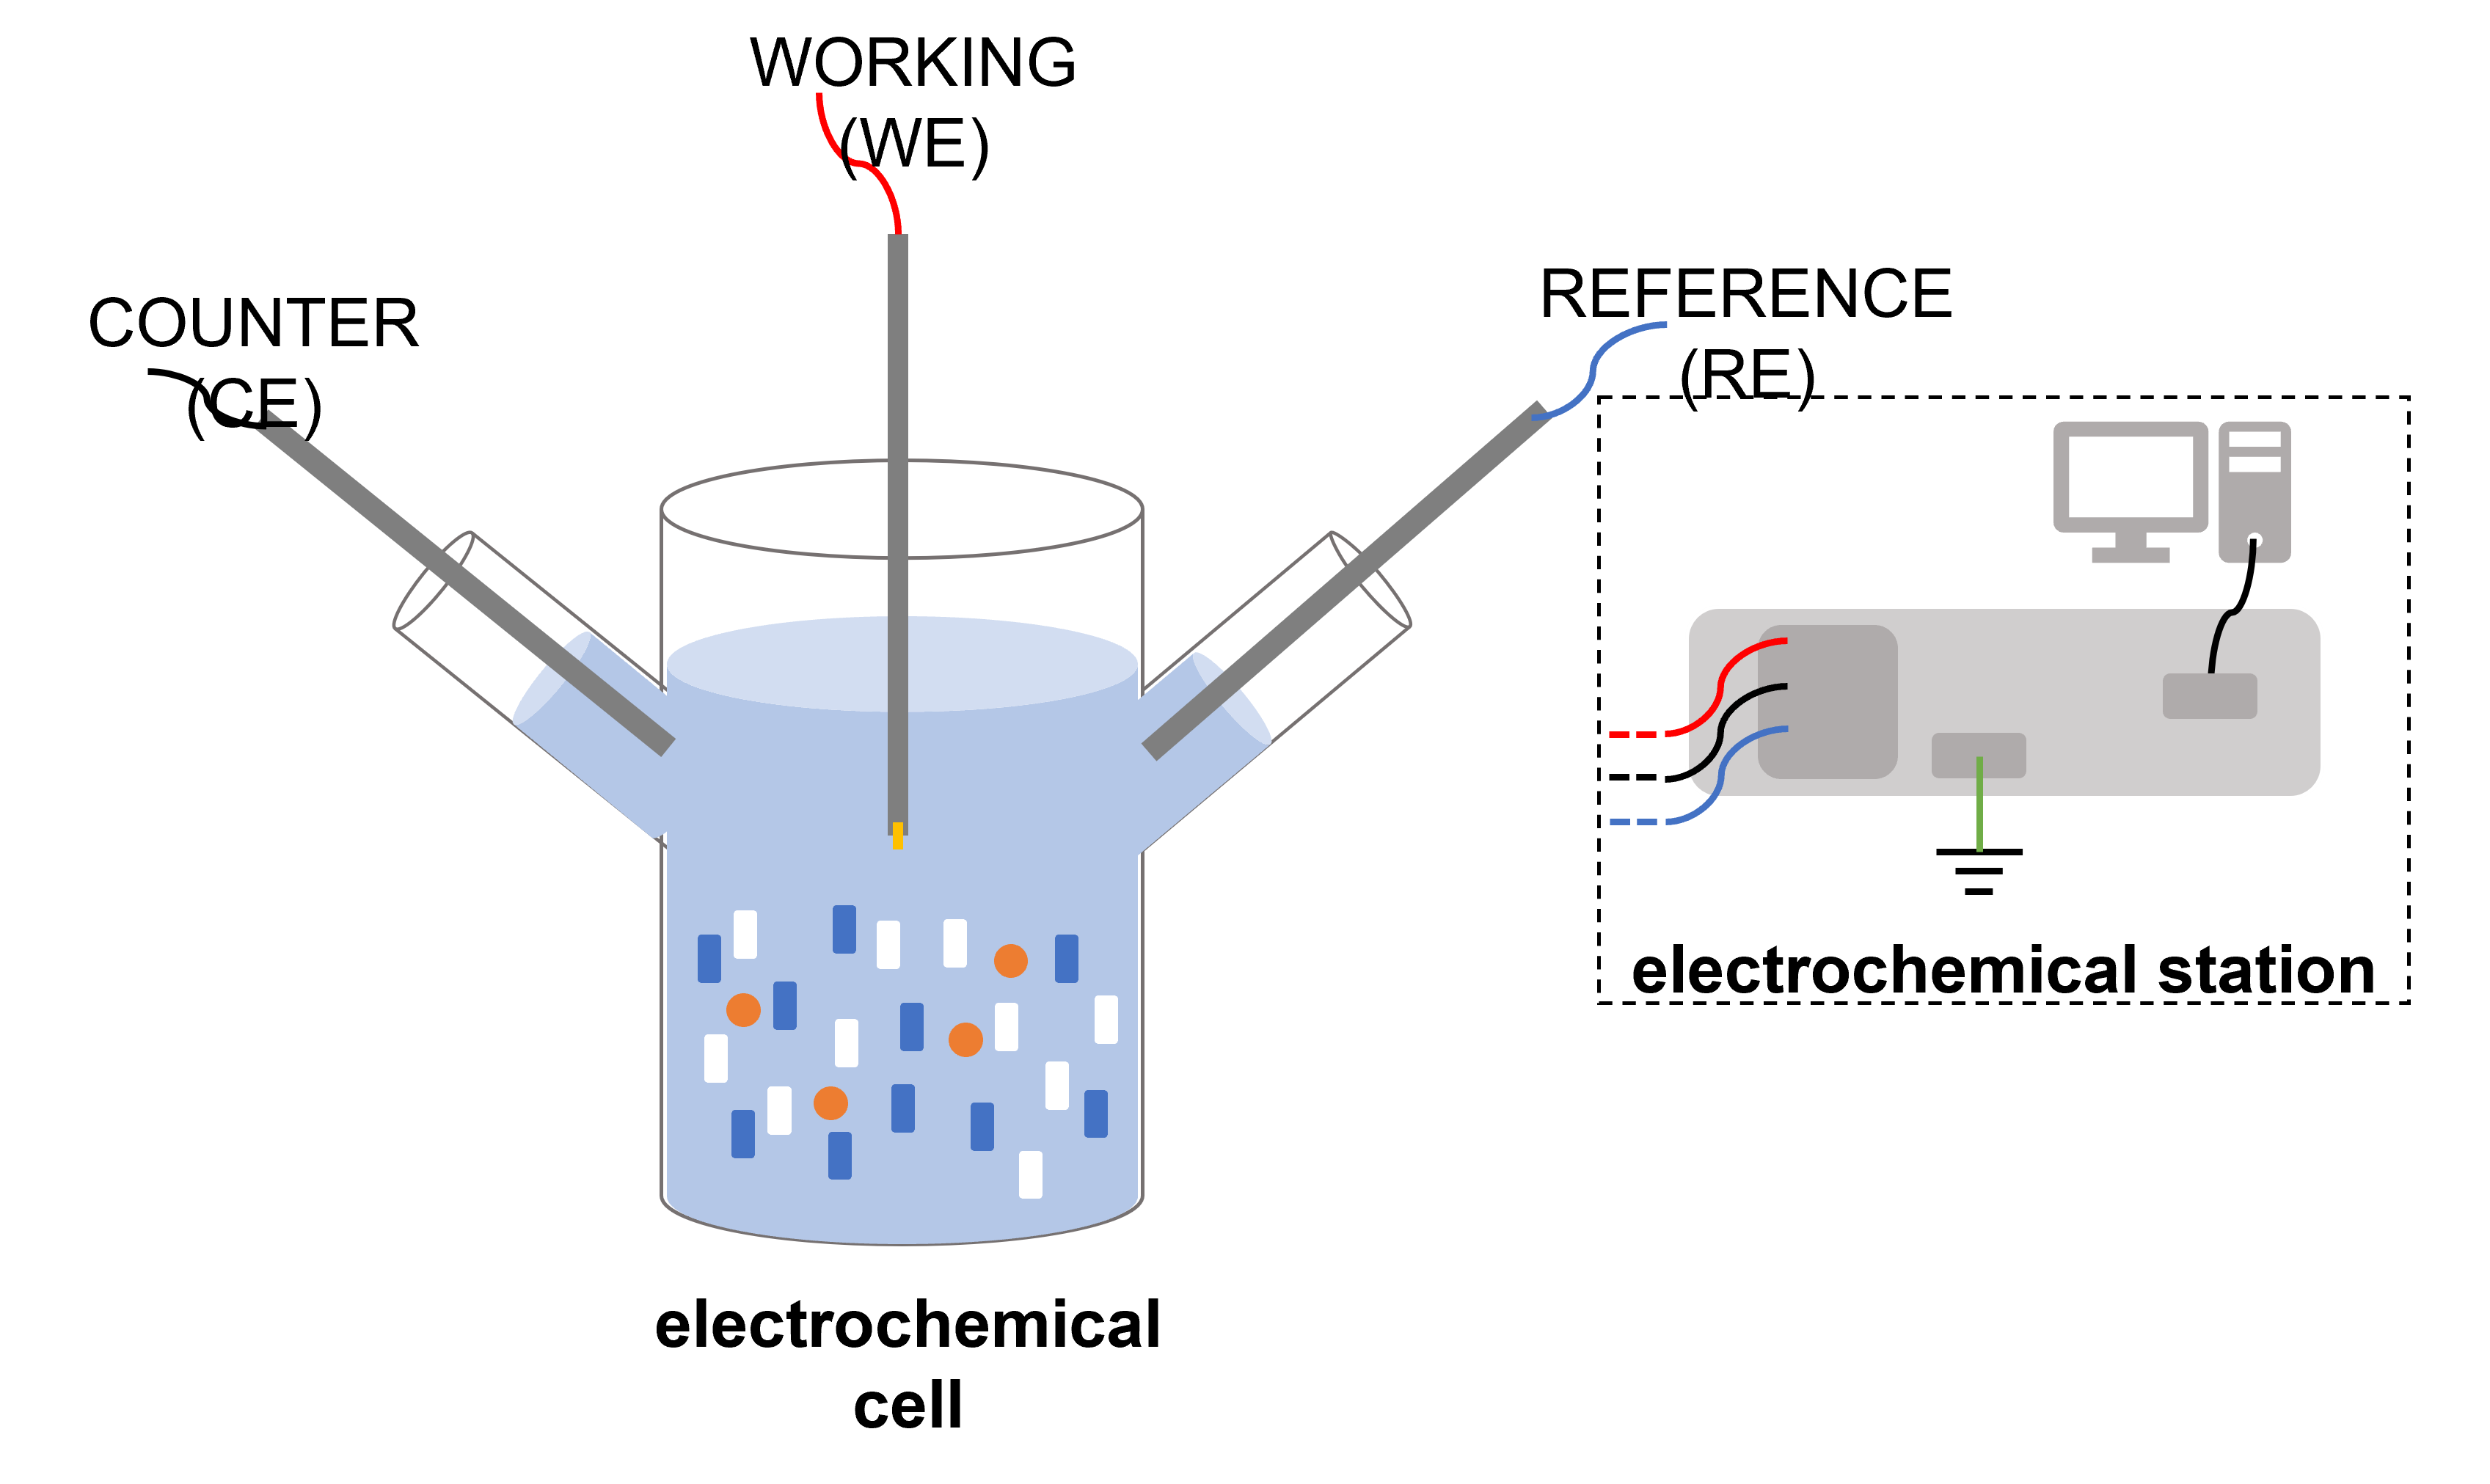
\includegraphics[width=.5\textwidth]{img/h2o2_setup.png}
    \caption{Electrochemical detection experimental setup for nitrite, hydrogen peroxide and lactate calibration}
    \label{fig:h2o2_setup}
\end{figure}
\noindent The experimental setup for hydrogen peroxide detection is shown in \autoref{fig:h2o2_setup}. Cyclic voltammetry was first performed in the blank buffer. This step is essentially a validation of the existence of PB in the reaction environment. \\\\
\noindent Chronoamperometry was performed following the cyclic voltammetry scan. Hydrogen peroxide was added to the reaction environment gradationally from 0$\mu$M to 300$\mu$M and reacted with Prussian blue. Current and time data were collected under each concentration; Coulometry was then performed for experimental validation.

%====================================================================================
\subsection{Lactate Investigations}
Ideally, our sensor would be able to detect lactate levels in the range of 0.5mmol/L to 4mmol/L; This would cover healthy and septic levels. Without modification, LOX sensors have a detection limit of 0.25mM where sites become saturated. To optimise the detection range, we need to increase the concentration at which saturation occurs. In this experiment,  Nafion, a sulfonated polymer, is coated onto the electrode surface, which leaves a negative charge in the solution, reducing the flux of lactate to the enzyme layer \cite{rathee2016biosensors} \cite{romero2010amperometric}. Further modifications to membrane thickness and enzyme type can increase our detection range. Electrodes were prepared from gold electrodes by coating with interference exclusion and enzyme hydrogel layers, see \autoref{app:lactate_protocol}.\\\\
The electrochemical cell was then set up using the lactate electrode as the working rotating disc electrode, platinum as the counter and Ag/AgCl as the working electrode with the configuration shown in \autoref{fig:h2o2_setup}.\\\\
RDE is important for enzyme sensors as it maximises the proportion of mass transport due to convection and allows for a fully defined flow pattern around the electrode \cite{nikolic2000theoretical}. Amperometry was then conducted at 0.7V and 400rpm on 7.4pH PBS solutions spiked with 0.2mM aliquots in the 0.0-3.0mM range and then 0.5mM aliquots in the 3.0-4.5mM range. \subsection{Aptamer Modelling}
\subsubsection{Numerical Inverse Laplace Algorithm}
The output current is sampled at discrete time points in chronoamperometric experiments on aptamer biosensors. We, therefore, need to adapt the NIL algorithm for discrete signals using a numerical linear least-squares approach.\\\\
For discrete signals, we can use the NIL transform to find the coefficients of the exponential decays (spectra $\mathbf{G}(k)$).
The algorithm aims to minimise the error between the model fit and the experimental data.
The discrete form of a general chronoamperometric signal can be represented as \autoref{Apt_discrete}:
\begin{equation}
    y(t_{i}) = \sum_{j=1}^{N} \mathbf{G}(k_{j})e^{-t_{i}k_{j}}
    \label{Apt_discrete}
\end{equation}
In matrix form \autoref{Apt_discrete} can be represented as:
$$ \mathbf{y = AG} $$
The minimisation becomes a linear least squares problem, which we solve using the Nelder Mead's method:
\begin{equation}
    min\lVert \mathbf{AG} - \mathbf{y}\lVert^{2}_{2}
    \label{discretething}
\end{equation}
where $\mathbf{G}$ $\in$ $\mathbf{R}^{N}$.\\\\
An additional regularizer is added to smooth the output solution.
\begin{equation}
    V(\alpha) = \lVert \mathbf{AG} - \mathbf{y}\lVert^{2}+\alpha^{2}\lVert \mathbf{r} - \mathbf{RG}\lVert  = min
\end{equation}
$\mathbf{R}$ considers prior knowledge of $\mathbf{G}(k)$. $\mathbf{r}$ represents the second derivative of $\mathbf{G}(k)$. Increasing the value of $\alpha$ favours smoother solutions, as they have smaller second derivative values. See \autoref{Aptamer_multiexp} for a detailed description of the mathematical implementation of the algorithm and \autoref{app:apt_mod} for the code to perform these simulations.\\\\
\subsubsection{Coarse-grained Modelling of Aptamers}
% \vspace{-.8cm}
To relate the electron transfer rates of the bound and unbound aptamer configurations ($k_{A}$, $k_{AT}$) to the distance between redox reporter (MB) and electrode surface, we develop a model of aptamers to predict the distribution of aptamer configurations.\\\\ 
Without considering the chemical or thermodynamic effects of base interactions within the aptamer \cite{feigon1996aptamer}, we assume the aptamers to be a freely-jointed chain where the chains can rotate with 3DOFs.
The persistence length is a mechanical property quantifying the bending stiffness of a polymer. For double-stranded DNA (dsDNA), persistence length is widely reported as 50 nm \cite{bloomfielduniversity,marko1995stretching}. The latest measurements of persistence length on single-stranded DNA (ssDNA) using atomic force microscopy shows a measurement of $1.98 \pm 0.72$nm \cite{roth2018measuring}, in the range of previously published values of 1.5 - 3nm \cite{murphy2004probing,chi2013persistence}. For pieces of ssDNA shorter than the persistence length, the molecule behaves like a rigid rod, while for pieces of the ssDNA that are much longer than the persistence length, the properties can be described statistically as a three-dimensional random walk.\\\\
For aptamers tested in the laboratory, their base numbers range from 50-100, corresponding to lengths of 17 and 34nm \cite{alberts2014molecular}, an order of magnitude larger than the persistence length of ssDNA. Therefore, we consider the aptamer as a freely-jointed chain with rigid segments of size $b = 2\zeta$ (where $\zeta$ is the persistence length, $b$ is the Kuhn length) \cite{strobl1997physics}.\\\\
In our model, we simulate random vectors in the spherical coordinate space for each rigid segment and extract the end-to-end distance from the redox reporter to the electrode surface. In cases where any of the rigid segments reach below the electrode surface ($z=0$), we instead take the absolute z-value (maintain the randomly generated theta value, and recalculate the phi value such that the Kuhn segment length is maintained) and continue the simulation. This, therefore, considers the redox reporter to bounce off the electrode. 3D simulations for 50, 100, and 200 bases (\autoref{Apt_sim}) are shown, where we plot the probability distribution for the end-to-end distance from the redox reporter to the electrode surface. \\\\
Extending the numerical simulation to 5E+06 simulations, the length distribution tends to be half-gaussian, centred at the electrode surface (z=0) (\autoref{L_dist}). The MATLAB code used to generate the stochastic models of the DNA is in \autoref{app:apt_mod}.
\begin{figure}[H]
    \centering
    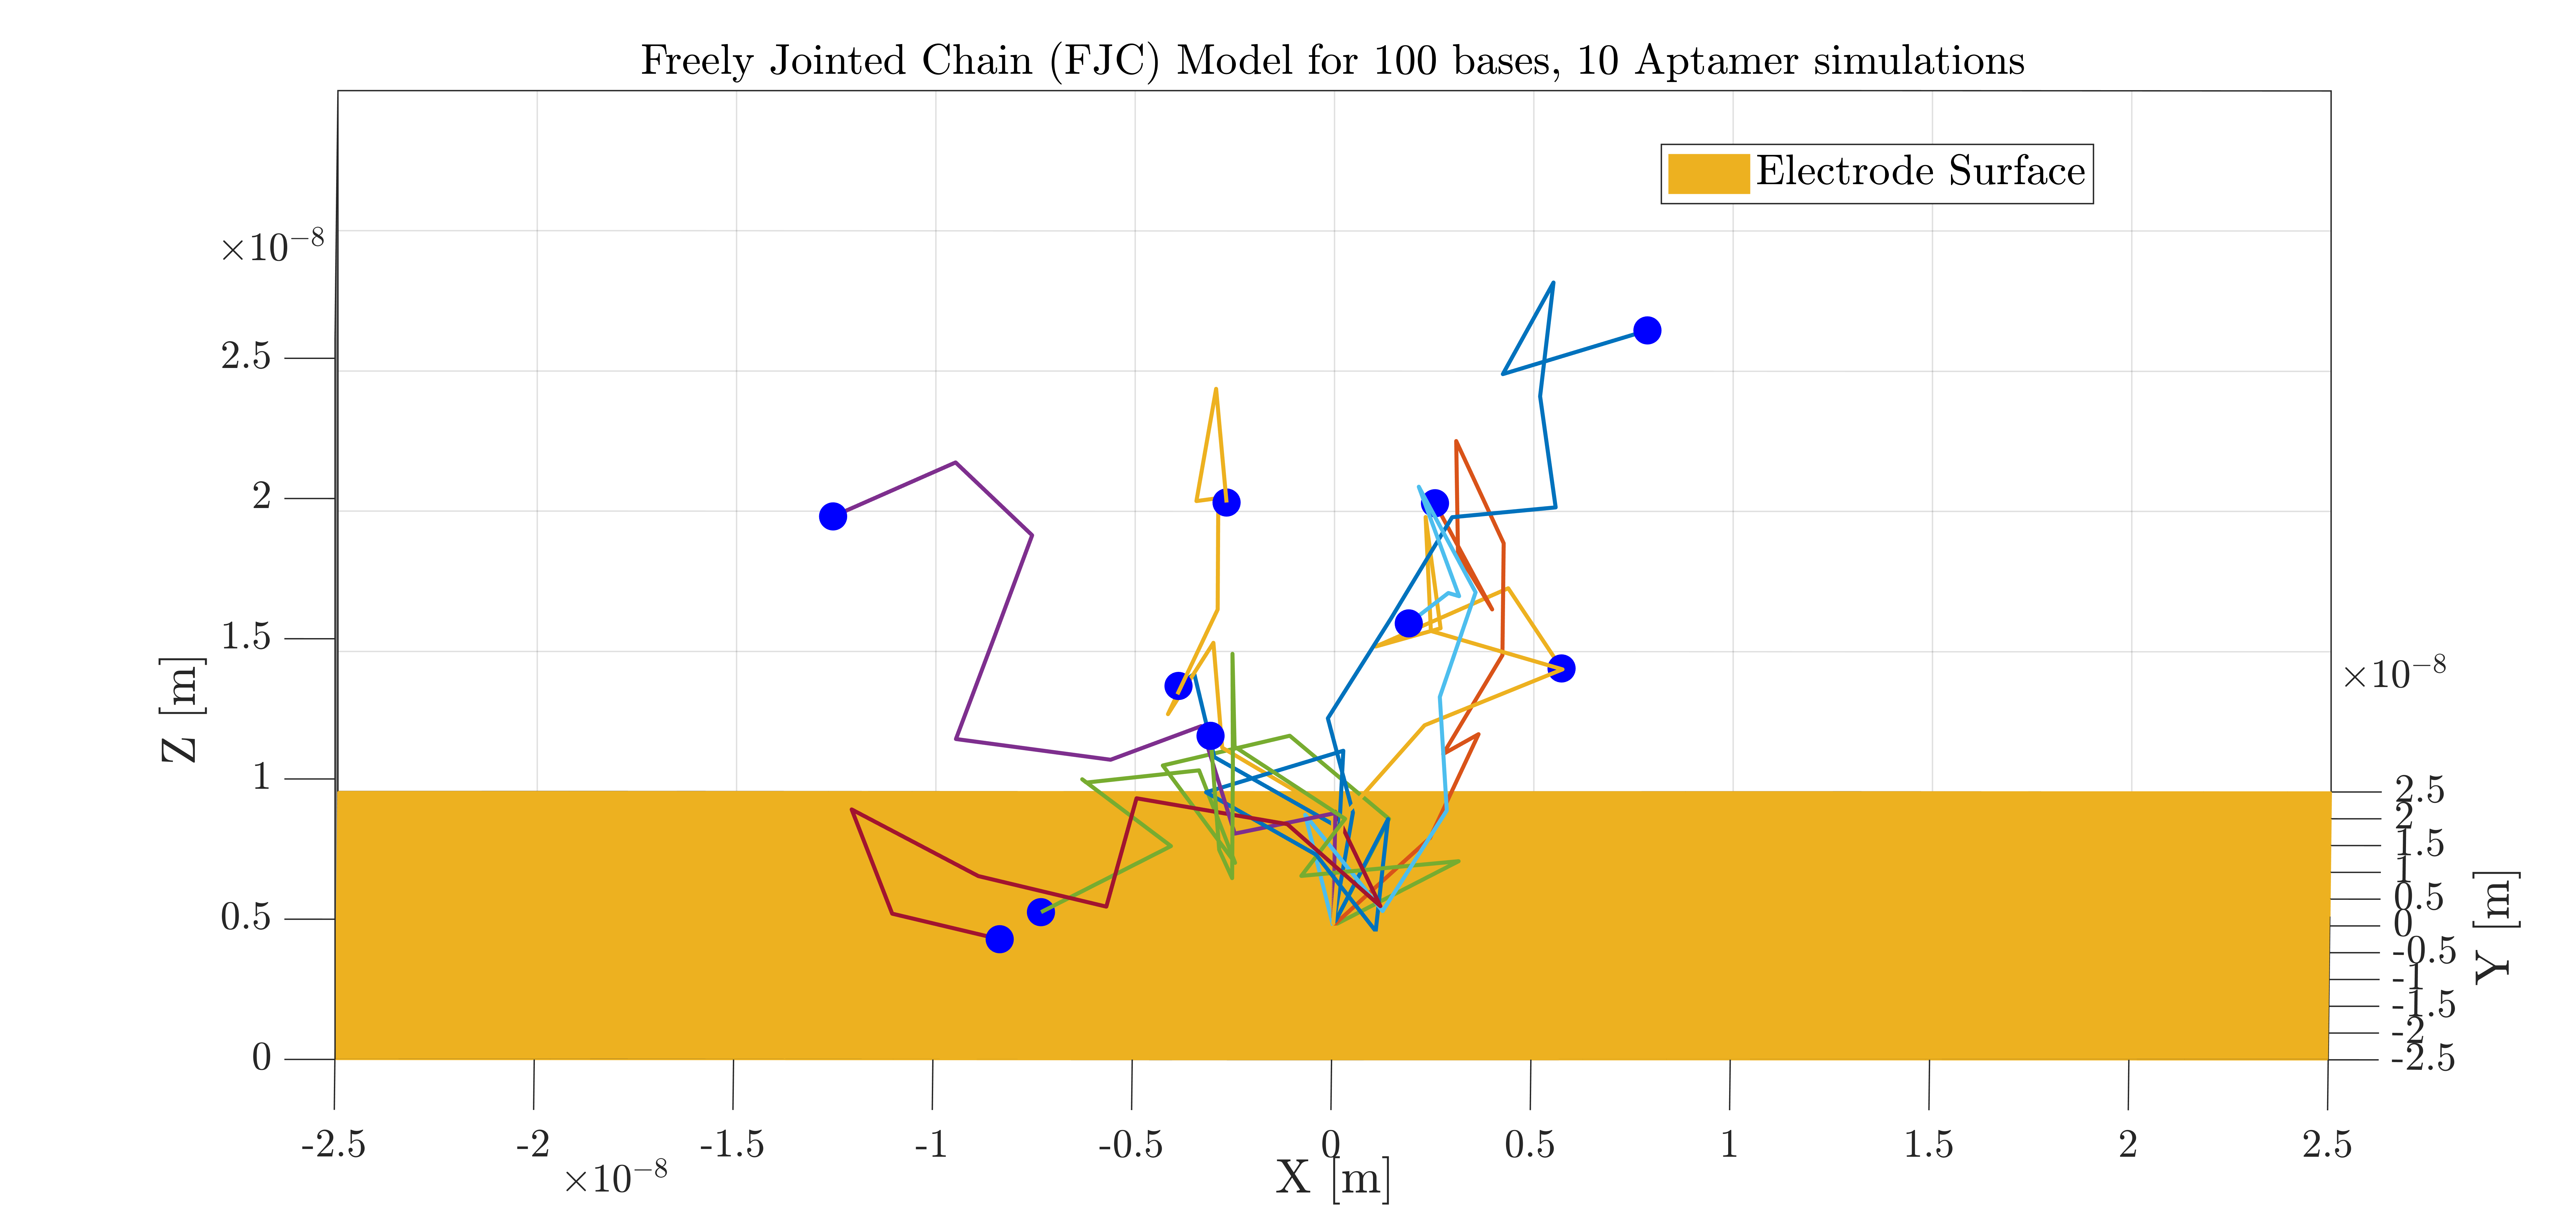
\includegraphics[width = 0.5\textwidth]{img/DNA_100_base_simulation_v1.png}
    \caption{Example plot of 10 random walk simulations for 100 bases with Kuhn length segements (b = 2$\zeta$, where $\zeta$ is the persistence length of the DNA}
    \label{Apt_sim}
\end{figure}
\begin{figure}[H]
    \centering
    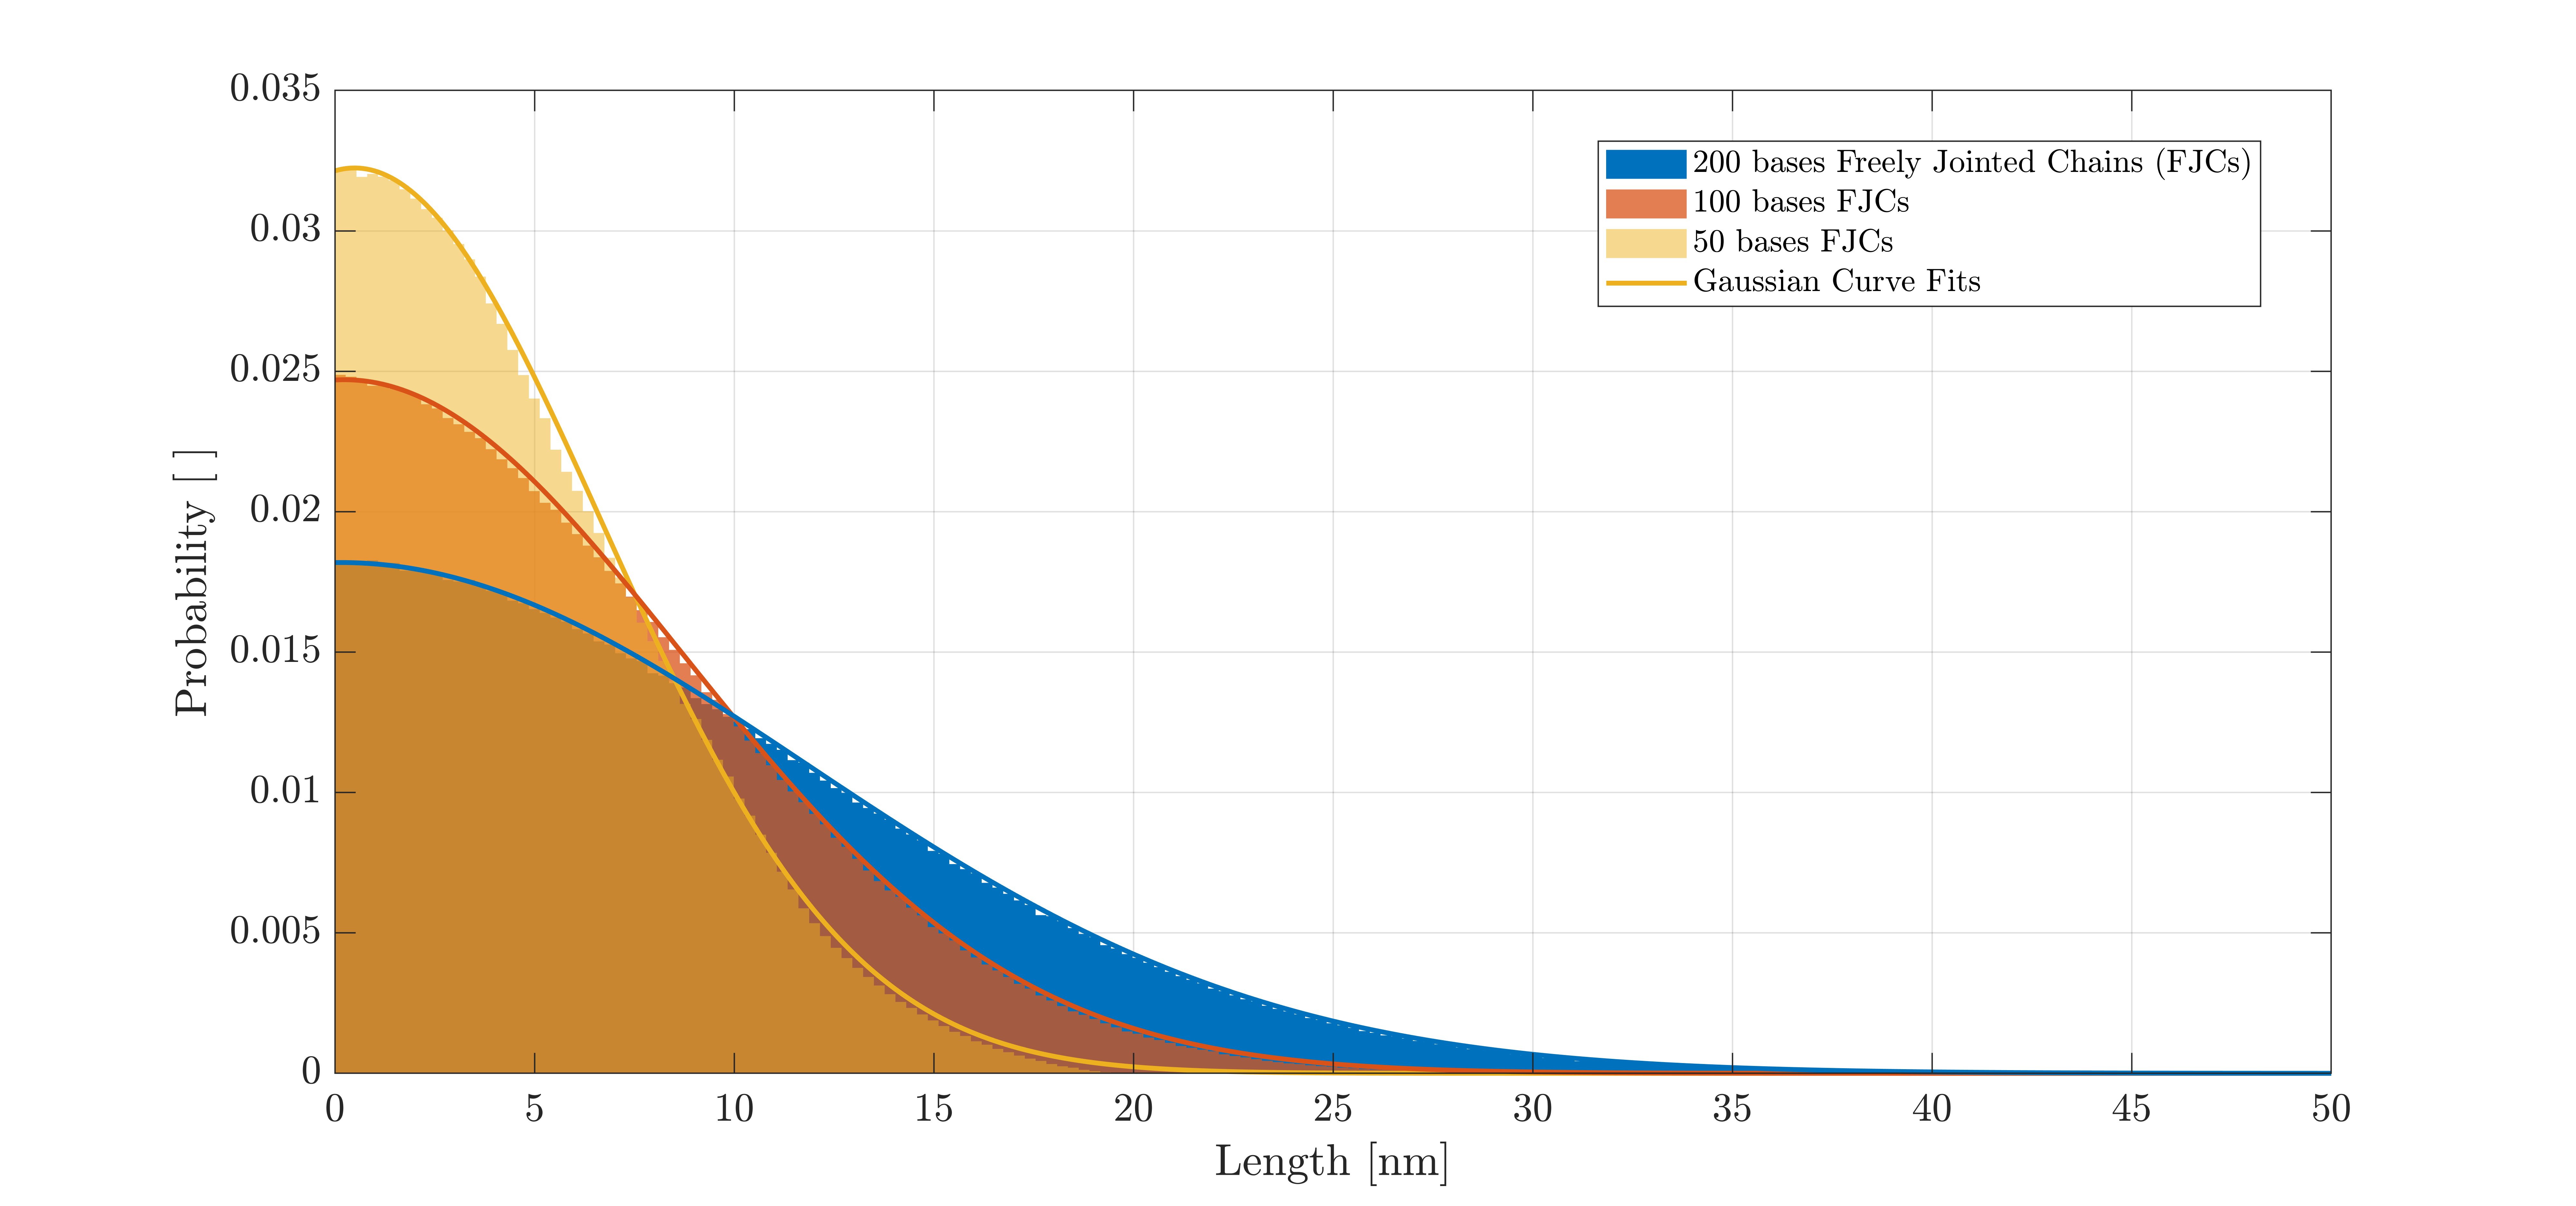
\includegraphics[width = 0.5\textwidth]{img/length_with_gaussians.png}
    \caption{Length probability distribution for aptamers of 200, 100, and 50 base lengths. Numerically simulated using the freely-jointed chain model. Assume aptamer bounces off electrode surface when z$\leq$0. Probability distribution approaches a half-gaussian distribution. Gaussian fits overlayed, with parameters shown in table 1}
    \label{L_dist}
\end{figure}

